\documentclass[11pt]{article}
\usepackage[margin=1in]{geometry}
\usepackage[T1]{fontenc}
\usepackage{lmodern,amsmath,amssymb,amsthm,tikz}
\usepackage[colorlinks=true,linkcolor=blue,citecolor=blue,urlcolor=blue,pdfauthor={P. Graham},pdftitle={A counterexample to two questions on acyclic polynomial roots}]{hyperref}
\newtheorem{theorem}{Theorem}
\newtheorem{lemma}[theorem]{Lemma}
\title{A counterexample to two questions on acyclic polynomial roots}
\author{P. Graham\\ \small\url{https://orcid.org/0009-0007-8493-1505}}
\date{October 31, 2026}
\begin{document}
\maketitle
\begin{abstract}
The acyclic polynomial of a graph counts its vertex subsets that induce forests, by their cardinality. We give a twelve-vertex graph whose acyclic polynomial has a real root smaller than every real root of the acyclic polynomial of the proposed extremal graph of Barton, Brown and Pike, and whose modulus exceeds that of every complex root of that polynomial. This answers both parts of their question on extremal acyclic roots negatively. Their work supplies the proposed graph, the complement of a four-cycle and a star, and a formula for its quartic polynomial. We replace that star by two three-leaf stars. The resulting polynomial differs only in its cubic coefficient. Exact sign evaluations and the triangle inequality separate the two root sets at radius eighty-six, without numerical root approximations. A Lean formalization proves the coefficient identities from induced-graph acyclicity and derives both failures of the universal assertions.

This work has not yet been reviewed by experts. The proofs, the Lean formalization and the text were produced by AI models (from OpenAI and Anthropic), working under the author's direction.
\end{abstract}
\medskip
\noindent\textbf{MSC 2020:} 05C31, 05C38.\quad
\textbf{Keywords:} acyclic polynomial, induced forest, graph polynomial roots.

\section{Introduction}
For a finite simple graph $H$ with vertex set $V(H)$, define its acyclic polynomial by
\[
 A(H,x)=\sum_{\substack{S\subseteq V(H)\\H[S]\text{ is a forest}}}x^{|S|}.
\]
Here $H[S]$ is the induced subgraph; the empty subset contributes $1$.
For example, every vertex subset of a forest on $m$ vertices induces a forest, so its acyclic polynomial is $(1+x)^m$.
Write $\overline H$ for the complement of $H$, and $\sqcup$ for disjoint union. Let $C_4$ be the four-cycle and $K_{1,k}$ the star with $k$ leaves. For $n\geq5$, put
\[
 J_n=\overline{C_4\sqcup K_{1,n-5}}.
\]
Thus the star in the definition of $J_n$ has $n-4$ vertices.

\begin{theorem}\label{thm:main}
Let $G=\overline{C_4\sqcup K_{1,3}\sqcup K_{1,3}}$. Then
\begin{align*}
 A(G,x)&=x^4+90x^3+66x^2+12x+1,\\
 A(J_{12},x)&=x^4+85x^3+66x^2+12x+1.
\end{align*}
There is a real root $r$ of $A(G,x)$ with $-100<r<-86$, whereas every complex root $z$ of $A(J_{12},x)$ satisfies $|z|<86$. Consequently, $r$ is smaller than every real root of $A(J_{12},x)$ and has greater modulus than every complex root of that polynomial.
\end{theorem}

Barton, Brown and Pike posed both extremal comparisons in their original preprint as Conjecture~1; the journal version states them as Question~2.17~\cite{BBP}. The question asks whether, for every $n\geq5$, $A(J_n,x)$ has a real root smaller than the real roots of all other acyclic polynomials of order $n$, and whether $J_n$ has an acyclic root of largest modulus at that order. Theorem~\ref{thm:main} refutes both assertions at $n=12$, which suffices to refute their universal quantification over $n$. Its two polynomials are distinct, as required for the first comparison. Minimality of the counterexample's order is not part of the theorem.

The construction and its quartic form build directly on Barton, Brown and Pike's $J_n$. Their Lemma~2.18 in the journal version gives
\[
 A(J_n,x)=x^4+\frac{n^2+5n-34}{2}x^3+
             \binom n2 x^2+nx+1.
\]
Splitting the seven-leaf star of $\overline{J_{12}}$ into two three-leaf stars increases the cubic coefficient while keeping the other coefficients fixed. The proof below explains that change by counting missing edges. A complete Lean proof also establishes the two coefficient identities directly from the definition of acyclicity.

\section{Proof overview}
The key finite step is to count induced forests after splitting the star. Both graphs have exactly one induced forest on four vertices and none on more vertices. For three vertices, a forest is precisely a triple containing a missing edge. Counting such triples gives cubic coefficients $90$ and $85$.

It then suffices to separate the roots at one radius. Opposite signs at $-100$ and $-86$ place a real root of the first polynomial to the left of $-86$. For the second, the leading term dominates the sum of the absolute values of all remaining terms whenever $|z|\geq86$. This yields a strict complex-root bound, which settles both questions simultaneously.

\begin{figure}[ht]
\centering
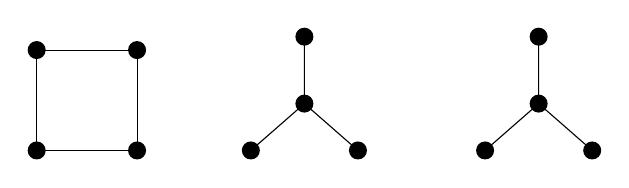
\begin{tikzpicture}[scale=0.85,every node/.style={circle,fill=black,inner sep=2.3pt}]
\coordinate (a) at (0,0); \coordinate (b) at (1.5,0);
\coordinate (c) at (1.5,1.5); \coordinate (d) at (0,1.5);
\draw (a)--(b)--(c)--(d)--(a);
\foreach \v in {a,b,c,d} \node at (\v) {};
\foreach \x in {4,7.5} {
\draw (\x,0.7)--(\x-0.8,0) (\x,0.7)--(\x+0.8,0) (\x,0.7)--(\x,1.7);
\node at (\x,0.7) {}; \node at (\x-0.8,0) {};
\node at (\x+0.8,0) {}; \node at (\x,1.7) {};
}
\end{tikzpicture}
\caption{The complement of $G$. The edges of $G$ are precisely the pairs absent from this drawing.}
\label{fig:complement}
\end{figure}

\section{Counting the induced forests}
\begin{lemma}\label{lem:count}
For $G$ and $J_{12}$ in Theorem~\ref{thm:main}, the acyclic polynomials are respectively
\[
 1+12x+66x^2+90x^3+x^4
 \quad\text{and}\quad
 1+12x+66x^2+85x^3+x^4.
\]
\end{lemma}
\begin{proof}
Every subset of at most two vertices induces a forest, giving coefficients $1$, $12$ and $\binom{12}{2}=66$ in both cases.

Let $F$ be the complement of either graph. A three-vertex subset induces a forest in $\overline F$ if and only if it contains an edge of $F$. Each edge of $F$ lies in ten triples. Because $F$ has no triangles, a triple contains at most two edges of $F$, and a triple with two edges is counted exactly twice. Hence the number of forest triples is
\[
 10|E(F)|-\sum_{v\in V(F)}\binom{\deg_F(v)}2.
\]
For $F=C_4\sqcup2K_{1,3}$, there are ten edges and the sum is $4+3+3=10$, giving $90$. For $F=C_4\sqcup K_{1,7}$, there are eleven edges and the sum is $4+\binom72=25$, giving $85$.

Next consider four vertices. If they meet at least three components of $F$, their induced graph in $\overline F$ contains a triangle. If they meet two components in two vertices each, it contains a four-cycle. If they meet two components in three vertices and one vertex, the triple cannot be a triangle in $F$, since $F$ is triangle-free. Thus some pair of the triple is an edge of $\overline F$; together with the vertex from the other component it forms a triangle in $\overline F$.

It follows that a forest on four selected vertices must lie within one component of $F$. Any four vertices of a star contain at least three leaves, which form a triangle in its complement. The four vertices of the $C_4$ component, however, induce two disjoint edges in $\overline F$. This is the unique forest subset of size four. A forest subset of size at least five would have more than one four-vertex subset, all inducing forests, a contradiction. This proves both identities.
\end{proof}

\section{Separating the roots}
\begin{lemma}\label{lem:disk}
Every complex root of $q(x)=x^4+85x^3+66x^2+12x+1$ has modulus less than $86$.
\end{lemma}
\begin{proof}
Let $z$ be a root and suppose $t=|z|\geq86$. From $q(z)=0$ and the triangle inequality,
\[
 t^4\leq85t^3+66t^2+12t+1.
\]
Dividing by $t^4>0$ and using $t\geq86$ gives
\[
 1\leq\frac{85}{t}+\frac{66}{t^2}+\frac{12}{t^3}+\frac1{t^4}
 \leq\frac{85}{86}+\frac{66}{86^2}+\frac{12}{86^3}+\frac1{86^4}<1.
\]
The final strict inequality follows from the exact integers
\[
 85\cdot86^3+66\cdot86^2+12\cdot86+1
 =54{,}553{,}929<54{,}700{,}816=86^4.
\]
This contradiction proves the bound.
\end{proof}

\begin{proof}[Proof of Theorem~\ref{thm:main}]
Lemma~\ref{lem:count} gives the two polynomials. Write $p(x)=A(G,x)$. Direct evaluation gives
\[
 p(-100)=10{,}658{,}801>0,\qquad p(-86)=-2{,}057{,}119<0.
\]
The intermediate value theorem supplies a real root $r\in(-100,-86)$. By Lemma~\ref{lem:disk}, every complex root $z$ of $A(J_{12},x)$ has $|z|<86<|r|$. In particular, every real root $s$ of that polynomial satisfies $s>-86>r$. Finally, the unequal cubic coefficients show that $A(G,x)\neq A(J_{12},x)$, completing both negative comparisons.
\end{proof}

\section{Formal verification}
The formal theorem \texttt{BBPSplitStar.endpoint} proves the two polynomial identities, the existence of a real root strictly between $-100$ and $-86$, the strict complex-root bound $86$, and the negations of both universal assertions. Its polynomial is a sum over vertex subsets whose induced simple graph satisfies Mathlib's standard acyclicity predicate. Its graphs are specified by their missing edges, agreeing with Figure~\ref{fig:complement}. The first universal assertion quantifies over distinct polynomials and follows Barton, Brown and Pike's strict wording; the endpoint's explicit root bounds also refute the non-strict reading, since $r<s$ for every real root $s$ of $A(J_{12},x)$. The second assertion quantifies over all complex roots of all graphs of the same order.

The finite proof checks every vertex subset and connects the resulting decisions to induced-graph acyclicity. The analytic proof uses continuity of polynomial evaluation and the complex norm triangle inequality. The entire endpoint is checked by the Lean kernel with the standard axioms of propositional extensionality, classical choice and quotient soundness, without compiled evaluation. Lean and Mathlib provide the underlying formal infrastructure~\cite{Lean,Mathlib}.

The accompanying formalization notes give the pinned dependencies and standard Lake commands. The default build includes the final theorem, statement checks, small graph examples and axiom guards. The elementary argument above establishes the mathematical result without requiring numerical root approximations.

\begin{thebibliography}{9}
\bibitem{BBP}
C. Barton, J. I. Brown and D. A. Pike,
\emph{Acyclic polynomials of graphs}, Australasian Journal of Combinatorics
82(2) (2022), 146--181. Question~2.17 and Lemma~2.18.
\url{https://ajc.maths.uq.edu.au/pdf/82/ajc_v82_p146.pdf}.
Original preprint: \href{https://arxiv.org/abs/2011.01735v1}{arXiv:2011.01735v1}, Conjecture~1; journal text also at \href{https://arxiv.org/abs/2011.01735v3}{arXiv:2011.01735v3}.
\bibitem{Lean}
L. de Moura and S. Ullrich,
\emph{The Lean 4 theorem prover and programming language},
Automated Deduction---CADE 28, LNCS 12699 (2021), 625--635.
\url{https://doi.org/10.1007/978-3-030-79876-5_37}.
\bibitem{Mathlib}
The mathlib Community,
\emph{The Lean mathematical library},
Proceedings of CPP 2020 (2020), 367--381.
\url{https://doi.org/10.1145/3372885.3373824}.
\end{thebibliography}
\end{document}
